\documentclass[tikz,border=8pt]{standalone}

\usepackage[T1]{fontenc}
\usepackage[utf8]{inputenc}
\usepackage{lmodern}
\usepackage{pgfplots}
\usetikzlibrary{arrows.meta}
\pgfplotsset{compat=1.18}

\definecolor{distBlue}{RGB}{30,90,200}
\definecolor{varRed}{RGB}{176,20,30}
\definecolor{cvarFill}{RGB}{252,190,190}

\begin{document}
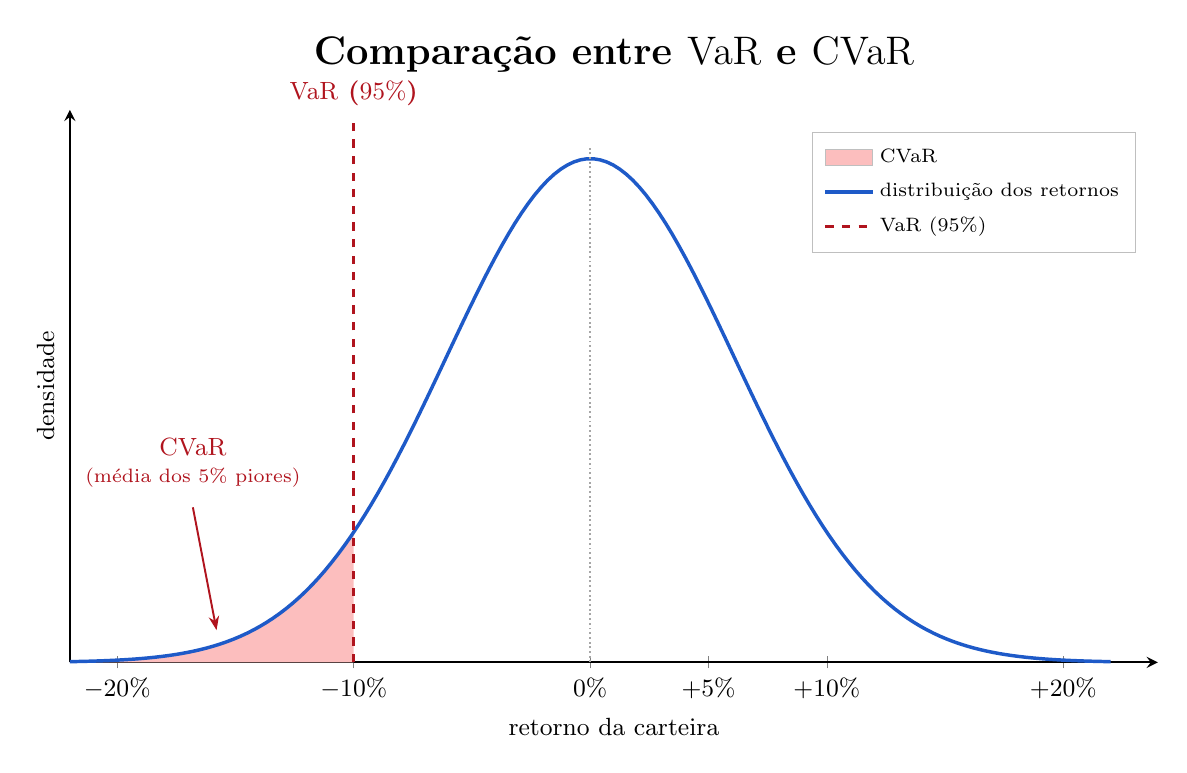
\begin{tikzpicture}
  \begin{axis}[
    width=15.4cm,
    height=8.6cm,
    title={Comparação entre $\mathrm{VaR}$ e $\mathrm{CVaR}$},
    title style={font=\bfseries\Large, yshift=4pt},
    xlabel={retorno da carteira},
    ylabel={densidade},
    xlabel style={font=\small},
    ylabel style={font=\small},
    xmin=-0.22, xmax=0.24,
    ymin=0, ymax=7.2,
    xtick={-0.20,-0.10,0,0.05,0.10,0.20},
    xticklabels={$-20\%$,$-10\%$,$0\%$,$+5\%$,$+10\%$,$+20\%$},
    ytick=\empty,
    axis lines=left,
    axis line style={thick},
    clip=false,
    legend style={
      at={(0.98,0.96)},
      anchor=north east,
      font=\scriptsize,
      cells={anchor=west},
      draw=black!25,
      fill=white,
      inner sep=4pt,
      row sep=2pt,
    },
    legend cell align=left,
    tick label style={font=\small},
    every axis plot/.append style={line join=round},
  ]

    \pgfmathdeclarefunction{gauss}{1}{%
      \pgfmathparse{exp(-((#1)^2)/(2*0.0608^2))/(0.0608*sqrt(2*pi))}%
    }

    \addplot[
      fill=cvarFill,
      draw=none,
      area legend,
      domain=-0.22:-0.10,
      samples=90,
    ] {gauss(x)} \closedcycle;
    \addlegendentry{$\mathrm{CVaR}$}

    \addplot[
      color=distBlue,
      line width=1.25pt,
      domain=-0.22:0.22,
      samples=160,
    ] {gauss(x)};
    \addlegendentry{distribuição dos retornos}

    \draw[varRed, dashed, line width=0.9pt]
      ({axis cs:-0.10,0}) -- ({axis cs:-0.10,7.05});
    \addlegendimage{varRed, dashed, line width=0.9pt}
    \addlegendentry{$\mathrm{VaR}$ ($95\%$)}

    \draw[black!35, densely dotted, line width=0.7pt]
      ({axis cs:0,0}) -- ({axis cs:0,6.7});

    \node[font=\small\bfseries, varRed, anchor=south]
      at (axis cs:-0.10,7.12) {$\mathrm{VaR}$ ($95\%$)};

    \node[align=center, font=\small, varRed, anchor=south]
      at (axis cs:-0.168,2.15) {$\mathrm{CVaR}$\\[-1pt]{\scriptsize (média dos $5\%$ piores)}};
    \draw[varRed, -{Stealth[length=5pt]}, line width=0.7pt]
      (axis cs:-0.168,2.02) -- (axis cs:-0.158,0.42);

  \end{axis}
\end{tikzpicture}
\end{document}
